\chapter{Tools}
Dieses Kapitel beschäftigt sich damit, wie eine Entwicklungsumgebung in Go und Swift aussehen könnte. 
% Welche Betriebssysteme werden unterstützt?
% Gibt es \gls{IDE} %integrierte Entwicklungsumgebungen?
% Welchen Umfang hat die Standardbibliothek?


\section{Entwicklungsumgebung}
Auf Github \cite[]{Github.Swift} werden für Swift die in \autoref{tab:UnterstützteBetriebssysteme} aufgeführten \textit{host development operationg systems} genannt.
In Go kann auf den in \autoref{tab:UnterstützteBetriebssysteme} gezeigten Plattformen entwickelt werden.

\begin{table}[H]
    \centering
    \begin{tabularx}{\textwidth}{ |X|X|X|X| }
    \hline 
    \rowcolor[gray]{0.75} \cellcolor{white} & \textbf{Windows} & \textbf{Linux} & \textbf{MacOS} \\
    \hline
    \cellcolor{Gray} \textbf{Go} Version 1.8.1 & Ab Windows XP & Ab Linux 2.6.23 & Ab MacOS X 10.8 \\
    \hline
    \cellcolor{Gray} \textbf{Swift} Version 3.1.1 &  & Ubuntu LTS und die letzte Ubuntu Version (Aktuell 16.10) & Xcode 8.3.2 \\
    \hline
    \end{tabularx}
    \caption{Unterstützte Betriebssysteme}
    \label{tab:UnterstützteBetriebssysteme}
\end{table}

Von \cite[]{TechnoPedia} wird eine Entwicklungsumgebung folgenderweise definiert.

\begin{quote}
\enquote{In software development, the development environment is a set of processes and tools that are used to develop a source code or program.}\cite[]{TechnoPedia}
\end{quote}

Eine einfache Entwicklungsumgebung besteht aus einem geeigneten Quelltext-Editor, Debugger und Compiler. Von \cite[]{NotUseIde} wird empfohlen auf eine Integrierte Entwicklungsumgebung (siehe \autoref{sec:IDE}) zu verzichten, um die hohe Lernkurve von Integrierten Entwicklungsumgebungen zu vermeiden.
Aus diesem Grund wurden alle Codebeispiele in dieser Arbeit mit einem Quelltext-Editor und den sprachspezifischen Werkzeugen entwickelt.
Als Quelltext-Editor wurde \textit{Visual Studio Code} eingesetzt. 
\textit{Visual Studio Code} zeichnet sich durch folgende Fähigkeiten aus:

\begin{itemize}
    \item Open Source
    \item Verfügbar für Windows, Linux und MacOS
    \item Durch \textit{Extensions} erweiterbar
    \item \textit{Extensions} für Go und Swift sind verfügbar
\end{itemize}

Die Installation von Swift und Go sowie Visual Studio Code wird hier nicht näher erläutert, da sich die Vorgehensweise von Version zu Version ändern kann.
Im folgenden wird die Einrichtung einer Arbeitsumgebung, im weiteren Verlauf auch \textit{Workspace} genannt, für Go und Swift erläutert.

Die offizielle Dokumention von Go \cite[]{GoDoc.Workspaces} äußert sich folgenderweise zum allgemeinen Aufbau einer Arbeitsumgebung für Go.

\begin{itemize}
    \item Go programmers typically keep all their Go code in a single workspace.
    \item \label{itm:GoWorkspaceSrc} A workspace contains many version control repositories (managed by Git, for example). 
    \item Each repository contains one or more packages.
    \item Each package consists of one or more Go source files in a single directory.
    \item The path to a package's directory determines its import path.
\end{itemize}

Der grundsätzliche Aufbau einer Arbeitsumgebung in Go ist in \autoref{fig:GoWorkspace} zu sehen. 

\begin{figure}[H]
    \centering
    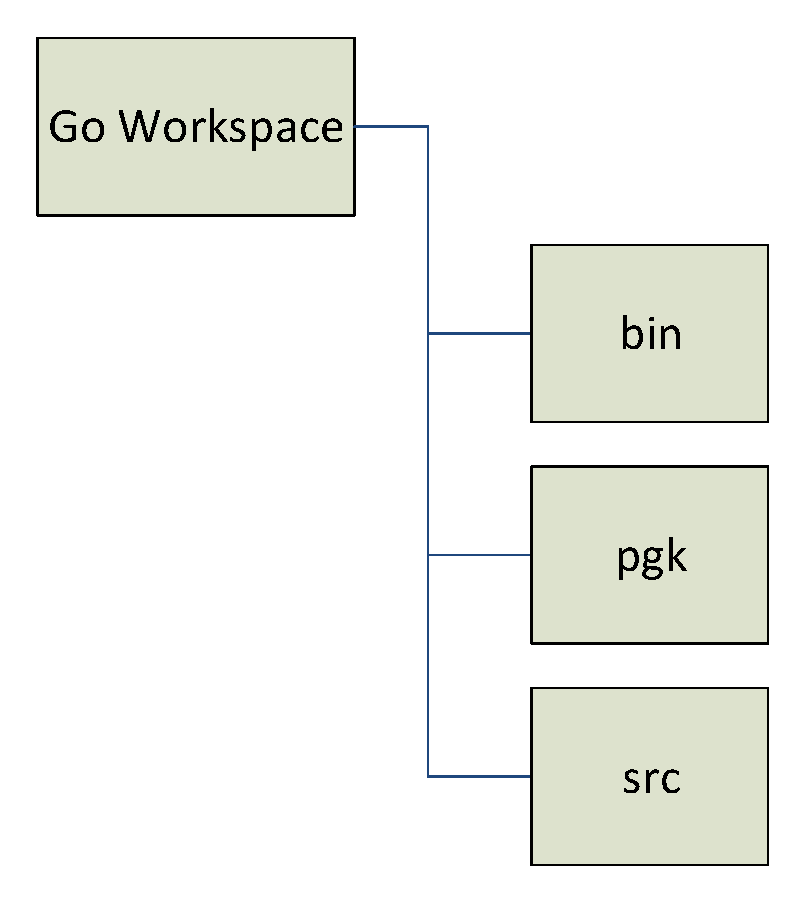
\includegraphics[height=6cm]{Images/GoWorkspace}
    \caption{Aufbau einer Arbeitsumgebung in Go}
    \label{fig:GoWorkspace}
\end{figure}

Wird Quelltext kompiliert, werden die vom Compiler erzeugten Binärdateien in den Ordner \textit{bin}, für ausführbare Progamme, und \textit{pkg}, für eigene Bibliotheken, abgelegt.

Im Ordner \textit{src} befindet sich der Quelltext, üblicherweise in Form von Repositorys eines Versionskontrollsystems.

Swift unterscheidet sich hier von Go. 
In Swift gibt es einzelne Arbeitsbereiche für jedes Projekt. 
Zudem ist es möglich sich diese Arbeitsbereiche mit dem Tool \textit{Swift Package Manager}, welches bei der Installation von Swift mitgeliefert wird, Arbeitsbereiche automatisiert anlegen zu lassen.

\begin{listing}[H]
\caption{Anwendung des \textit{Swift Package Managers} Quelle: \cite[S.22]{Hoffman.2017}}
\label{lst:SwiftPackageManager}
\begin{Commandline}
mkdir PMExample

cd PMExample

swift package init
\end{Commandline}
\end{listing}

\autoref{fig:SwiftWorkspace} zeigt den Aufbau des Arbeitsbereichs, nach Ausführen des \textit{Swift Package Managers} mit dem Befehl \textit{init}. 

\begin{figure}[H]
    \centering
    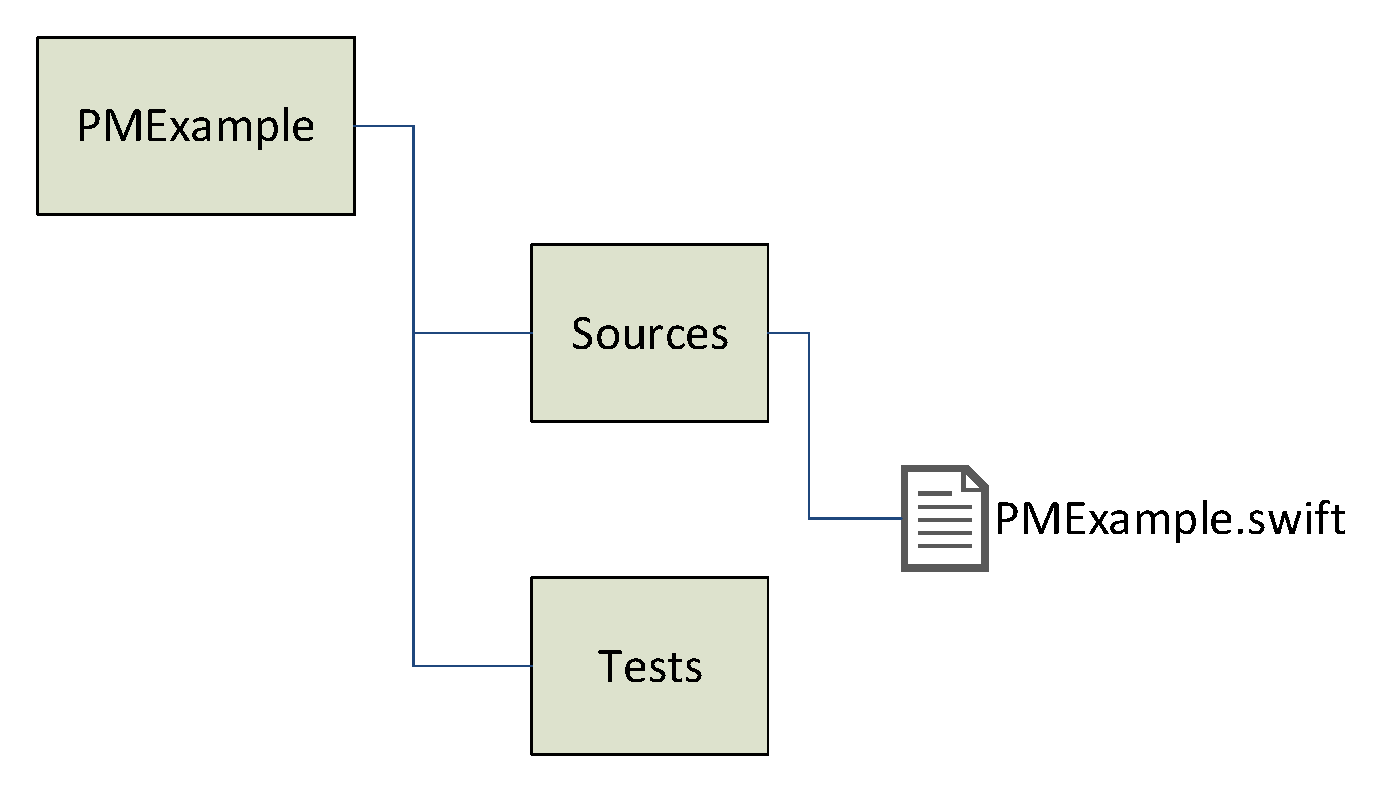
\includegraphics[height=6cm]{Images/SwiftWorkspace}
    \caption{Ein mit dem Swift Package Manager angelegter Workspace}
    \label{fig:SwiftWorkspace}
\end{figure}

Der \textit{Swift Package Manager} legt in dem in \autoref{lst:SwiftPackageManager} angelegten Verzeichnis die Verzeichnisse \textit{Sources} u. \textit{Tests} an.
Zusätzlich wird die Datei \textit{PMExample.swift} im Verzeichnis \textit{Sources} angelegt.

\section{Integrierte Entwicklungsumgebungen}
\label{sec:IDE}
Dieser Abschnitt soll einen Marktüberblick über die für Swift und Go vefügbaren integrierten Entwicklungsumgebungen bieten.
Eine integrierte Entwicklungsumgebung vereint laut \cite[]{TechnoPedia} die folgenden Fähigkeiten.

\begin{itemize}
    \item Editieren von Quelltext
    \item Build-Prozess ausführen
    \item Tests ausführen
    \item Debugging
\end{itemize}

Derzeit gibt es mit \textit{LiteIDE} (https://github.com/visualfc/liteide) nur eine richtige integrierte Entwicklungsumgebung für Go.
\textit{LiteIDE} ist Open Source und ist auf folgenden Plattformen verfügbar:

\begin{itemize}
    \item Windows 
    \item Linux
    \item MacOS X ab Version 10.6
    \item FreeBSD ab Version 9.2
    \item OpenBSD ab Version 5.6
\end{itemize}

Die Firma Jetbrains hat angekündigt mit \textit{Gogland}\cite[]{Gogland} eine integrierte Entwicklungsumgebung für Swift auf den Markt zu bringen, siehe \cite[]{Gogland.Heise}.
\textit{Gogland} befindet sich aktuell noch im \textit{Early Access Program}, einer Vorabversion.

Swift ist zwar für Linux und MacOS verfügbar, jedoch gibt es mit XCode nur eine integrierte Entwicklungsumgebung für MacOS.

\section{Standardbibliothek}
Apple beschreibt die Standardbibliothek von Swift mit folgendem Satz.
\begin{quote}
\enquote{The Swift language is relatively small, because many common types, functions, and operators that appear virtually everywhere in Swift code are actually defined in the Swift standard library.} \cite[S.427]{Apple.2017}
\end{quote}

Von \cite[S.184]{Kennedy.2016} wird ein Vorteil bei Verwendung der Go Standardbibliothek genannt. 

\begin{quote}
\enquote{By using packages from the standard library, you make it easier to manage your code and ensure that it’s reliable. This is because you
don’t have to worry if your program is going to break between release cycles, nor do
you have to manage third-party dependencies.} \cite[S.185]{Kennedy.2016}
\end{quote}

Die Standardbibliothek, sowohl von Go als auch Swift, ist also ein wichtiger Bestandteil der Programmiersprache. 
Laut \cite[S.185]{Kennedy.2016} beinhaltet die Standardbibliothek von Go über 100 Packages, welche in 38 Kategorien unterteilt sind.

Mit der dritten Version von Swift gelang es den Entwicklern den Quelltext von Swift \textit{source-compatible} zu machen.
Dies bedeutet, dass Swift Quelltext auf allen unterstützen Plattformen (siehe \autoref{tab:UnterstützteBetriebssysteme}) kompiliert werden kann \cite[S.8]{Hoffman.2017}.
Eine ausführliche Standardbibliothek ist wichtig und minimiert die Abhängigkeit von externen Bibliotheken.



